\documentclass{ximera}

\usepackage[T1]{fontenc}
\usepackage{stix2}
\usepackage{gillius}
\usepackage{resizegather}
%\usepackage{rsfso} fancy cal
\DeclareMathAlphabet{\mathcal}{OMS}{cmsy}{m}{n} %less fancy cal


\usepackage{multicol}


\usepackage{tikz-cd}
\usepackage{tkz-euclide} %% compass
\usetkzobj{all}  %% tkzCompass
\tikzset{>=stealth}
\tikzcdset{arrow style=tikz}
\usetikzlibrary{math} %% for assigning variables
%\usetikzlibrary{fadings}

\usepackage{colortbl,boldline,makecell} %% group tables


\usepackage[sans]{dsfont}

\usepackage{stmaryrd,pifont}

\graphicspath{
  {./}
  {fields/}
  }     



\let\oldbibliography\thebibliography%% to compact bib
\renewcommand{\thebibliography}[1]{%
  \oldbibliography{#1}%
  \setlength{\itemsep}{0pt}%
}
\renewcommand\refname{} %% no name needed!


\DefineVerbatimEnvironment{macaulay2}{Verbatim}{numbers=left,frame=lines,label=Macaulay2,labelposition=topline}

\DefineVerbatimEnvironment{gap}{Verbatim}{numbers=left,frame=lines,label=GAP,labelposition=topline}

%%% This next bit of code defines all our theorem environments
\makeatletter
\let\c@theorem\relax
\let\c@corollary\relax
%\let\c@example\relax
\makeatother

\let\definition\relax
\let\enddefinition\relax

\let\theorem\relax
\let\endtheorem\relax

\let\proposition\relax
\let\endproposition\relax

\let\exercise\relax
\let\endexercise\relax

\let\question\relax
\let\endquestion\relax

\let\remark\relax
\let\endremark\relax

\let\corollary\relax
\let\endcorollary\relax


\let\example\relax
\let\endexample\relax

\let\warning\relax
\let\endwarning\relax

\let\lemma\relax
\let\endlemma\relax


\let\algorithm\relax
\let\endalgorithm\relax
\usepackage{algpseudocode}

\newtheoremstyle{SlantTheorem}{\topsep}{\topsep}%%% space between body and thm
		{\slshape}                      %%% Thm body font
		{}                              %%% Indent amount (empty = no indent)
		{\bfseries\sffamily}            %%% Thm head font
		{}                              %%% Punctuation after thm head
		{3ex}                           %%% Space after thm head
		{\thmname{#1}\thmnumber{ #2}\thmnote{ \bfseries(#3)}}%%% Thm head spec
\theoremstyle{SlantTheorem}
\newtheorem{theorem}{Theorem}
%\newtheorem{definition}[theorem]{Definition}
%\newtheorem{proposition}[theorem]{Proposition}
%% \newtheorem*{dfnn}{Definition}
%% \newtheorem{ques}{Question}[theorem]
%% \newtheorem*{war}{WARNING}
%% \newtheorem*{cor}{Corollary}
%% \newtheorem*{eg}{Example}
\newtheorem*{remark}{Remark}
\newtheorem*{touchstone}{Touchstone}
\newtheorem{corollary}{Corollary}[theorem]
\newtheorem*{warning}{WARNING}
\newtheorem{example}[corollary]{Example}
\newtheorem{lemma}[theorem]{Lemma}




\newtheoremstyle{Definition}{\topsep}{\topsep}%%% space between body and thm
		{}                              %%% Thm body font
		{}                              %%% Indent amount (empty = no indent)
		{\bfseries\sffamily}            %%% Thm head font
		{}                              %%% Punctuation after thm head
		{3ex}                           %%% Space after thm head
		{\thmname{#1}\thmnumber{ #2}\thmnote{ \bfseries(#3)}}%%% Thm head spec
\theoremstyle{Definition}
\newtheorem{definition}[theorem]{Definition}



\let\algorithm\relax
\let\endalgorithm\relax
\newtheoremstyle{Alg}{\topsep}{\topsep}%%% space between body and thm
		{}                              %%% Thm body font
		{}                              %%% Indent amount (empty = no indent)
		{\bfseries\sffamily}            %%% Thm head font
		{}                              %%% Punctuation after thm head
		{3ex}                           %%% Space after thm head
		{\thmname{#1}\thmnumber{ #2}\thmnote{ \bfseries(#3)}}%%% Thm head spec
\theoremstyle{Alg}
\newtheorem*{algorithm}{Algorithm}
\newtheorem*{construction}{Construction}




\newtheoremstyle{Exercise}{\topsep}{\topsep} %%% space between body and thm
		{}                           %%% Thm body font
		{}                           %%% Indent amount (empty = no indent)
		{\bfseries\sffamily}         %%% Thm head font
		{)}                          %%% Punctuation after thm head
		{ }                          %%% Space after thm head
		{\thmnumber{#2}\thmnote{ \bfseries(#3)}}%%% Thm head spec
\theoremstyle{Exercise}
\newtheorem{exercise}[corollary]{}%[theorem]

%% \newtheoremstyle{Question}{\topsep}{\topsep} %%% space between body and thm
%% 		{\bfseries}                  %%% Thm body font
%% 		{3ex}                        %%% Indent amount (empty = no indent)
%% 		{}                           %%% Thm head font
%% 		{}                           %%% Punctuation after thm head
%% 		{}                           %%% Space after thm head
%% 		{\thmnumber{#2}\thmnote{ \bfseries(#3)}}%%% Thm head spec
\newtheoremstyle{Question}{3em}{3em} %%% space between body and thm
		{\large\bfseries}                           %%% Thm body font
		{}                           %%% Indent amount (empty = no indent)
		{}                         %%% Thm head font
		{}                          %%% Punctuation after thm head
		{0em}                          %%% Space after thm head
		{}%%% Thm head spec
\theoremstyle{Question}
\newtheorem*{question}{}






\renewcommand{\tilde}{\widetilde}
\renewcommand{\bar}{\overline}
\renewcommand{\hat}{\widehat}
\newcommand{\N}{\mathbb N}
\newcommand{\Z}{\mathbb Z}
\newcommand{\R}{\mathbb R}
\newcommand{\Q}{\mathbb Q}
\newcommand{\C}{\mathbb C}
\newcommand{\V}{\mathbb V}
\newcommand{\I}{\mathbb I}
\newcommand{\A}{\mathbb A}
\renewcommand{\o}{\mathbf o}
\newcommand{\iso}{\simeq}
\newcommand{\ph}{\varphi}
\newcommand{\Cf}{\mathcal{C}}
\newcommand{\IZ}{\mathrm{Int}(\Z)}
\newcommand{\dsum}{\oplus}
\newcommand{\directsum}{\bigoplus}
\newcommand{\union}{\bigcup}
\newcommand{\subgp}{\leq}
\newcommand{\normal}{\trianglelefteq}
\renewcommand{\i}{\mathfrak}
\renewcommand{\a}{\mathfrak{a}}
\renewcommand{\b}{\mathfrak{b}}
\newcommand{\m}{\mathfrak{m}}
\newcommand{\p}{\mathfrak{p}}
\newcommand{\q}{\mathfrak{q}}
\newcommand{\dfn}[1]{\textbf{#1}\index{#1}}
\let\hom\relax
\DeclareMathOperator{\mat}{Mat}
\DeclareMathOperator{\ann}{Ann}
\DeclareMathOperator{\h}{ht}
\DeclareMathOperator{\tr}{tr}
\DeclareMathOperator{\hom}{Hom}
\DeclareMathOperator{\Span}{Span}
\DeclareMathOperator{\spec}{Spec}
\DeclareMathOperator{\maxspec}{MaxSpec}
\DeclareMathOperator{\aut}{Aut}
\DeclareMathOperator{\ass}{Ass}
\DeclareMathOperator{\lcm}{lcm}
\DeclareMathOperator{\ff}{Frac}
\DeclareMathOperator{\im}{Im}
\DeclareMathOperator{\syz}{Syz}
\DeclareMathOperator{\gr}{Gr}
\DeclareMathOperator{\multideg}{multideg}
\renewcommand{\ker}{\mathop{\mathrm{Ker}}\nolimits}
\newcommand{\coker}{\mathop{\mathrm{Coker}}\nolimits}
\newcommand{\lps}{[\hspace{-0.25ex}[}
\newcommand{\rps}{]\hspace{-0.25ex}]}
\newcommand{\into}{\hookrightarrow}
\newcommand{\onto}{\twoheadrightarrow}
\newcommand{\tensor}{\otimes}
\newcommand{\x}{\mathbf{x}}
\newcommand{\X}{\mathbf X}
\newcommand{\Y}{\mathbf Y}
\renewcommand{\k}{\boldsymbol{\kappa}}
\renewcommand{\emptyset}{\varnothing}
\renewcommand{\qedsymbol}{$\blacksquare$}
\renewcommand{\l}{\ell}
\newcommand{\1}{\mathds{1}}
\newcommand{\lto}{\mathop{\longrightarrow\,}\limits}
\newcommand{\rad}{\sqrt}
\newcommand{\hf}{H}
\newcommand{\hs}{H\!S}
\newcommand{\hp}{H\!P}
\renewcommand{\vec}{\mathbf}
\let\temp\phi
\let\phi\varphi
\let\eulerphi\temp


\renewcommand{\epsilon}{\varepsilon}
\renewcommand{\subset}{\subseteq}
\renewcommand{\supset}{\supseteq}
\newcommand{\macaulay}{\normalfont\textsl{Macaulay2}}
\newcommand{\GAP}{\normalfont\textsf{GAP}}
\newcommand{\invlim}{\varprojlim}
\renewcommand{\le}{\leqslant}
\renewcommand{\ge}{\geqslant}
\newcommand{\valpha}{{\boldsymbol\alpha}}
\newcommand{\vbeta}{{\boldsymbol\beta}}
\newcommand{\vgamma}{{\boldsymbol\gamma}}
\newcommand{\dotp}{\bullet}
\newcommand{\lc}{\normalfont\textsc{lc}}
\newcommand{\lt}{\normalfont\textsc{lt}}
\newcommand{\lm}{\normalfont\textsc{lm}}
\newcommand{\from}{\leftarrow}
\newcommand{\transpose}{\intercal}
\newcommand{\grad}{\boldsymbol\nabla}
\newcommand{\curl}{\boldsymbol{\nabla\times}}
\renewcommand{\d}{\, d}
\newcommand{\<}{\langle}
\renewcommand{\>}{\rangle}

%\renewcommand{\proofname}{Sketch of Proof}


\renewenvironment{proof}[1][Proof]
  {\begin{trivlist}\item[\hskip \labelsep \itshape \bfseries #1{}\hspace{2ex}]\upshape}
{\qed\end{trivlist}}

\newenvironment{sketch}[1][Sketch of Proof]
  {\begin{trivlist}\item[\hskip \labelsep \itshape \bfseries #1{}\hspace{2ex}]\upshape}
{\qed\end{trivlist}}



\makeatletter
\renewcommand\section{\@startsection{paragraph}{10}{\z@}%
                                     {-3.25ex\@plus -1ex \@minus -.2ex}%
                                     {1.5ex \@plus .2ex}%
                                     {\normalfont\large\sffamily\bfseries}}
\renewcommand\subsection{\@startsection{subparagraph}{10}{\z@}%
                                    {3.25ex \@plus1ex \@minus.2ex}%
                                    {-1em}%
                                    {\normalfont\normalsize\sffamily\bfseries}}
\makeatother

%% Fix weird index/bib issue.
\makeatletter
\gdef\ttl@savemark{\sectionmark{}}
\makeatother


\makeatletter
%% no number for refs
\newcommand\frontstyle{%
  \def\activitystyle{activity-chapter}
  \def\maketitle{%
    \addtocounter{titlenumber}{1}%
                    {\flushleft\small\sffamily\bfseries\@pretitle\par\vspace{-1.5em}}%
                    {\flushleft\LARGE\sffamily\bfseries\@title \par }%
                    {\vskip .6em\noindent\textit\theabstract\setcounter{problem}{0}\setcounter{sectiontitlenumber}{0}}%
                    \par\vspace{2em}
                    \phantomsection\addcontentsline{toc}{section}{\textbf{\@title}}%
                  }}
\makeatother



\NewEnviron{annotate}{\vspace{-.3cm}\small \itshape \BODY \vspace{.3cm}}


%%%% TIKZ STUFF

%% N-GON code
\tikzset{
    pics/tikzngon/.style={
        code={
        \tikzmath{\xx = #1;\rr=1.7;}
        \draw[ultra thick,rounded corners=.05mm] ({\rr*sin(0*360/\xx)},{\rr*cos(0*360/\xx)})
        \foreach \x in {-1,0,...,\xx}
        {
        -- ({\rr*sin(\x*360/\xx)},{\rr*cos(\x*360/\xx)})
        }
           -- cycle;
  }}}

%% N-GON code (even)
\tikzset{
    pics/tikzegon/.style={
        code={
        \tikzmath{\xx = #1;\rr=1.7;}
        \draw[ultra thick,rounded corners=.05mm] ({\rr*sin(0*360/\xx+180/\xx)},{\rr*cos(0*360/\xx+180/\xx)})
        \foreach \x in {-1,0,...,\xx}
           {
           -- ({\rr*sin(\x*360/\xx+180/\xx)},{\rr*cos(\x*360/\xx+180/\xx)}) 
           }
           -- cycle;
  }}}




%% N-CLOCK code
\tikzset{
    pics/tikznclock/.style={
        code={
        \tikzmath{\xx = #1;\rr=1.7;\dd=.4;}
        \foreach \x in {1,...,\xx}
        \pgfmathtruncatemacro{\xy}{\x-1}
           {
             \node[circle,fill=black,inner sep=0pt, minimum size=13pt,text=white]
             at ({(\rr-\dd)*sin((\x-1)*360/(\xx)},{(\rr-\dd)*cos((\x-1)*360/\xx}) {\normalfont\bfseries\sffamily\small {\xy}};
           }
  \draw[thick] (0,0) circle (\rr);
  }}}



%% barcode from
%% https://tex.stackexchange.com/questions/6895/is-there-a-good-latex-package-for-generating-barcodes
%% NOT CURRENTLY USED!


\def\barcode#1#2#3#4#5#6#7{\begingroup%
  \dimen0=0.1em
  \def\stack##1##2{\oalign{##1\cr\hidewidth##2\hidewidth}}%
  \def\0##1{\kern##1\dimen0}%
  \def\1##1{\vrule height10ex width##1\dimen0}%
  \def\L##1{\ifcase##1\bc3211##1\or\bc2221##1\or\bc2122##1\or\bc1411##1%
    \or\bc1132##1\or\bc1231##1\or\bc1114##1\or\bc1312##1\or\bc1213##1%
    \or\bc3112##1\fi}%
  \def\R##1{\bgroup\let\next\1\let\1\0\let\0\next\L##1\egroup}%
  \def\G##1{\bgroup\let\bc\bcg\L##1\egroup}% reverse
  \def\bc##1##2##3##4##5{\stack{\0##1\1##2\0##3\1##4}##5}%
  \def\bcg##1##2##3##4##5{\stack{\0##4\1##3\0##2\1##1}##5}%
  \def\bcR##1##2##3##4##5##6{\R##1\R##2\R##3\R##4\R##5\R##6\11\01\11\09%
    \endgroup}%
  \stack{\09}#1\11\01\11\L#2%
  \ifcase#1\L#3\L#4\L#5\L#6\L#7\or\L#3\G#4\L#5\G#6\G#7%
    \or\L#3\G#4\G#5\L#6\G#7\or\L#3\G#4\G#5\G#6\L#7%
    \or\G#3\L#4\L#5\G#6\G#7\or\G#3\G#4\L#5\L#6\G#7%
    \or\G#3\G#4\G#5\L#6\L#7\or\G#3\L#4\G#5\L#6\G#7%
    \or\G#3\L#4\G#5\G#6\L#7\or\G#3\G#4\L#5\G#6\L#7%
  \fi\01\11\01\11\01\bcR}


\author{Bart Snapp}

\title{Subgroups}

\begin{document}
\begin{abstract}
  Subgroups are subsets of groups that are also groups. 
\end{abstract}
\maketitle


If a group $H$ is contained inside of another group $G$, and both
group use the same operation, then we say $H$ is a \textit{subgroup}
of $G$.




\begin{definition}\label{D:subgp}
  Let $(G,\star)$ be a group, a subset $S\subset G$ is a \dfn{subgroup} if
  \begin{enumerate}
  \item $S \ne \emptyset$,
  \item $a,b\in S \Rightarrow a\star b\in S$,
  \item $a\in S \Rightarrow a^{-1}\in S$.
  \end{enumerate}
  We denote subgroups by writing $S\subgp G$.\index{S<G@$S\subgp G$}
\end{definition}


\begin{exercise}
  Below we have listed pairs of the form $S\subset G$. In which of
  these pairs is $S$ a subgroup of $G$?  Select all that apply.
  \begin{selectAll}
  \choice[correct]{$\{x^2:x\in\Z_2\}\subset \Z_2$}
  \choice[correct]{$\{3x:x\in\Z\}\subset \Z$}
  \choice{$\Z_4= \{0,1,2,3\}\subset \Z$}
  \choice{$\{x^3:x\in\Z\}\subset \Z$}
  \choice[correct]{$\{0,6\}\subset \Z_{12}$}
  \choice{$\Z_p^\times\subset \Z_p$}
  \end{selectAll}
\end{exercise}




\begin{exercise}\index{nZ@$n\Z$}
  Let $n\Z = \{n\cdot x : x\in \Z\}$. Prove that $n\Z\subgp \Z$.
\end{exercise}


\begin{exercise}
  Let $(G,\star)$ be a group and $S$ be a subgroup of $G$. Prove that
  $(S,\star)$ is a group.
\end{exercise}

\begin{exercise}
  Prove that if $(G,\star)$ is a group and $S\subset G$ is a \textbf{finite}
  subset of $G$ such that
  \begin{enumerate}
  \item $S \ne \emptyset$,
  \item $a,b\in S \Rightarrow a\star b\in S$,
  \end{enumerate}
  then $S$ is a subgroup of $G$.
\end{exercise}


\begin{example}[Lattice diagram for $\boldsymbol{\pmb\Z_6}$]
  We can visualize the subgroup structure of a group with a lattice
  diagram. Here is the lattice diagram for $\Z_6$:
  \[
   \begin{tikzcd}
    & \Z_6 \ar[ld,-]  \ar[rdd,-] &       \\
    \<2\> \ar[rdd,-] &  &\\
   & &  \< 3\> \ar[ld,-]        \\   
    & \<0\> &
   \end{tikzcd}
   \]
  Typically we draw a lattice diagram with the largest subgroups at
  the top. The lines mean that there is containment between the groups.
\end{example}

\begin{exercise}
  Find the order of each subgroup of $\Z_6$.
\end{exercise}

\begin{example}[Lattice diagram for $\boldsymbol{\pmb\Z_8}$]
  Here is the subgroup lattice diagram for $\Z_8$:
  \[
  \begin{tikzcd}
    \Z_8  \ar[d,-] \\
    \<2\> \ar[d,-] \\
    \<4\> \ar[d,-] \\   
    \<0\> 
  \end{tikzcd}
  \]
\end{example}

\begin{exercise}
  Find the order of each subgroup of $\Z_8$.
\end{exercise}

\begin{exercise}
  Draw lattice diagrams for $\Z_n$ for $n=2,3\dots, 12$.
\end{exercise}




\begin{example}[Lattice diagram for $\boldsymbol{D_3}$]\index{symmetries!of the equilateral triangle}
  Here is the subgroup lattice diagram for $D_3$:
  \[
  \begin{tikzcd}
    & D_3 \ar[rdd,-]\ar[rrdd,-]\ar[rrrdd,-]  \ar[ld,-] & & &      \\
    \<r\> \ar[rdd,-]       &       &  & &  \\
    &       &  \< f\> \ar[ld,-]   &  \< rf\> \ar[lld,-]       &  \< r^2f\> \ar[llld,-]        \\   
    & \<e\> & & &
  \end{tikzcd}
  \]
\end{example}



\begin{example}[Witnessing the subgroups of $\boldsymbol{D_3}$]
  Consider the following picture:
  \[
  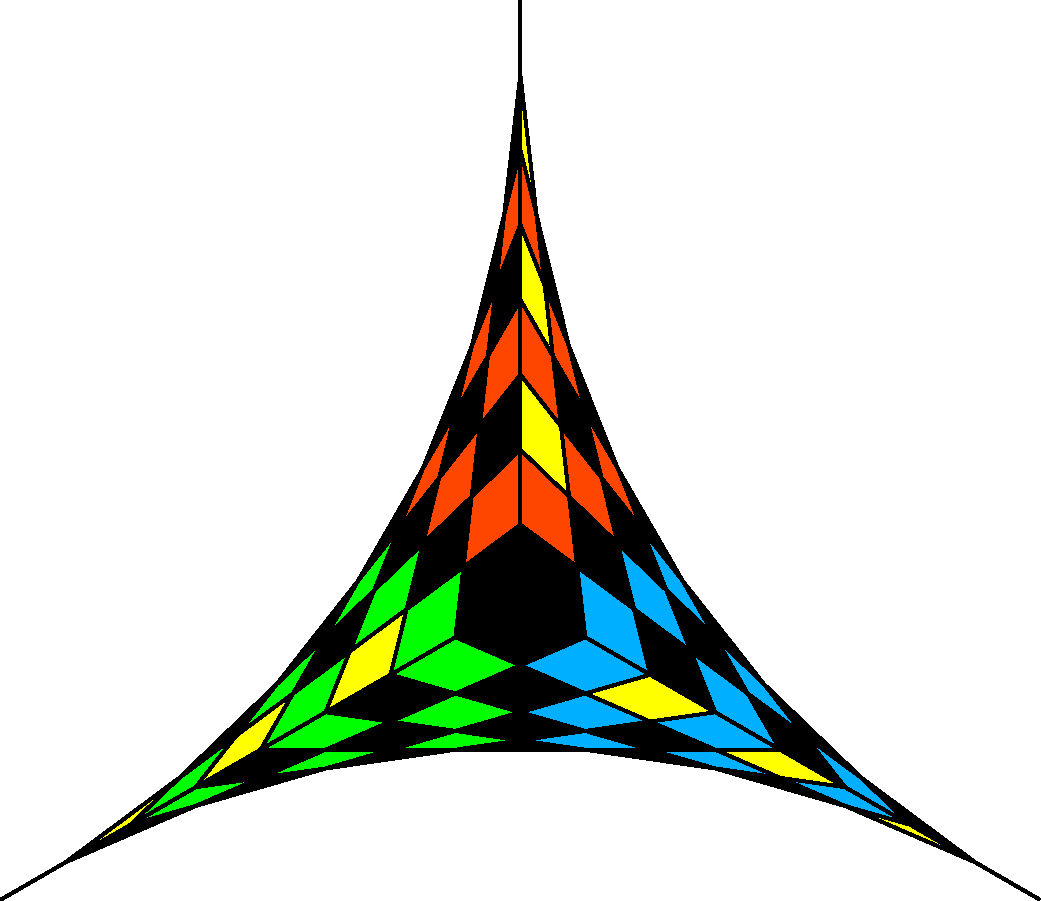
\includegraphics[width=.6\textwidth]{threeSubgp.pdf}
  \]
  If we associate yellow as black and all the other colors as the
  color white, then our picture has a symmetry group equal to $D_3$.

  
  If we associate all non-yellow colors as the color white, then our
  picture has a symmetry group equal to $\< r \>\subgp D_3$.

  
  If we associate yellow and black, and any two other non-yellow
  colors as the color white, then our picture will have a symmetry
  group equal to $\< f\> \subgp D_3$, $\< rf\> \subgp D_3$, or $\<
  r^2f\> \subgp D_3$.
\end{example}





\begin{exercise}
  Find the order of each subgroup of $D_3$.
\end{exercise}





\begin{example}[Lattice diagram for $\boldsymbol{D_4}$]
  Here is the subgroup lattice diagram for $D_4$:
  \[
  \begin{tikzcd}
    &    & D_4 \ar[rd,-] \ar[d,-] \ar[ld,-] &       \\
    &\<r^2,f\>  \ar[rd,-] \ar[d,-] \ar[ld,-]& \<r \>  \ar[d,-]     & \<r^2,rf\> \ar[ld,-] \ar[d,-] \ar[rd,-]\\
    \<f\>\ar[rrd,-]& \<r^2f\> \ar[rd,-]&\< r^2\> \ar[d,-]  &   \<rf\> \ar[ld,-]& \<r^3f\>\ar[lld,-]     \\   
&     & \<e\> &  &
  \end{tikzcd}
  \]  
\end{example}

\begin{exercise}
  Find the order of each subgroup of $D_4$.
\end{exercise}



\begin{example}[Lattice diagram for $\boldsymbol{Q_8}$]\index{quaternion group}
  Here is the subgroup lattice diagram for $Q_8$:
  \[
  \begin{tikzcd}
    & Q_8 \ar[rd,-] \ar[d,-] \ar[ld,-] &       \\
    \<i\>  \ar[rd,-] & \<j\>  \ar[d,-]     & \<k\> \ar[ld,-]\\
    &\< -1\> \ar[d,-]&        \\   
    & \<1\> &
  \end{tikzcd}
  \]
\end{example}


\begin{exercise}
  Find the order of each subgroup of $Q_8$.
\end{exercise}



\begin{example}[Nonisomorphic groups with similar lattice diagrams]
  Note, different groups may have the same lattice diagram structure.
  Again, consider the lattice for $\Z_6$:
  \[
  \begin{tikzcd}
    & \Z_6 \ar[ld,-]  \ar[rdd,-] &       \\
    \<2\> \ar[rdd,-] &  &\\
   & &  \< 3\> \ar[ld,-]        \\   
    & \<0\> &
  \end{tikzcd}
  \] 
  Now check out the lattice diagram for $\Z_{15}$:
  \[
  \begin{tikzcd}
        & \Z_{15} \ar[ld,-]  \ar[rdd,-] &       \\
    \<3\> \ar[rdd,-] &  &\\
   & &  \< 5\> \ar[ld,-]        \\   
    & \<0\> &
      \end{tikzcd}
  \]
\end{example}






Let's show the lattice diagram for one more group.

\begin{example}[Lattice diagram for $\boldsymbol{A_4}$]\index{alternating group}
  Setting $\sigma = (1 \ 2 \ 3)$ and $\tau = (2 \ 3 \ 4)$, here is the
  subgroup lattice diagram for $A_4$:
  \[
  \begin{tikzpicture}
  \node[scale=.6] at (0,0) {\begin{tikzcd}
                   &   & & A_4   \ar[lld,-] \ar[rdd,-] \ar[rrdd,-]  \ar[rrrdd,-]  \ar[rrrrdd,-]   & &  & &        \\
                   & \<\sigma\tau, \sigma^2\tau^2\> \ar[ldd,-] \ar[dd,-] \ar[rdd,-] &  &              & &  & &  \\
                   &                                  &            &   & \<\sigma\> \ar[ldd,-]& \<\tau\> \ar[lldd,-] & \<\ \tau\sigma^2\> \ar[llldd,-]& \< \sigma \tau\sigma^2 \>\ar[lllldd,-]       \\
   \<\sigma\tau\>\ar[drrr,-]  & \<\sigma^2\tau^2\> \ar[drr,-] & \<\sigma^2\tau\sigma^2\> \ar[dr,-]& & &  & &    \\
                   &                               &   & \< e\>       & & & &  
  \end{tikzcd}};
  \end{tikzpicture}
  \]
\end{example}


\begin{exercise}
  Find the order of each subgroup of $A_4$.
\end{exercise}

\begin{exercise}
  Draw a subgroup lattice diagram for $\mathcal{T}_{12}$.
\end{exercise}


\begin{theorem}[Subgroup criterion]\label{T:sc}\index{subgroup criterion}
  Let $G$ be a group, a nonempty $S\subset G$ is a subgroup if and
  only if
  \[
  a,b\in S \quad \Rightarrow \quad ab^{-1}\in S.
  \]
  \begin{proof}
    $(\Rightarrow)$ Follows from the definition of a subgroup.

    $(\Leftarrow)$ Suppose for all $a,b\in S$, we know that
    $ab^{-1}\in S$. We must show that $ab\in S$ and that every element
    has an inverse.

    Suppose that $a\in S$. This means $aa^{-1} = e\in S$.  Now since
    $e,b\in S$, $eb^{-1}\in S$, so $b^{-1}\in S$.  Finally, since
    $a,b^{-1}\in S$, $ab\in S$. We see that $S\subgp G$.
  \end{proof}
\end{theorem}


\begin{exercise}
  Prove that $SO(n)$ is a subgroup of $O(n)$.
\end{exercise}


\begin{exercise}\label{E:center}
  Let $G$ be a group, define the \dfn{center} of $G$ as
  \[
  Z(G):=\{g\in G: \text{$gx=xg$ for all $x\in G$}\}.
  \]
  Prove that $Z(G)$ is a subgroup of $G$.
  \begin{hint}
    First prove that if $G$ is an element that commutes with every
    element of $G$, then $g^{-1}$ also commutes with every element of
    $G$.
  \end{hint}
\end{exercise}


\begin{exercise}
  Let $G$ be a group, define the \dfn{normalizer} of $S$ in $G$ as
  \[
  N_G(S):=\{g\in G: \text{$gSg^{-1} = S$}\},
  \]
  where $gSg^{-1}:=\{g sg^{-1}:s\in S\}$. Prove that $N_G(S)$ is a
  subgroup of $G$.
\end{exercise}



\begin{exercise}
  Let $S$ and $T$ be subgroups of $(G,\star)$. Define
  \[
  S\star T := \{ s\star t: \text{$s\in S$ and $t\in T$}\}.
  \]
  Prove that $S\star T\subgp G$ if and only if $S\star T = T\star S$.
\end{exercise}



%% \begin{exercise}
%%   Consider the polynomial $x_1+x_2-x_3$. Prove that the set
%%   permutations on $\{x_1,x_2,x_3\}$ that fi
%% \end{exercise}



\begin{exercise}
  Let $H_1,H_2,\dots,H_n$ be subgroups of a group $G$. Prove that
  \[
  \bigcap_{i=1}^n H_i \subgp G.
  \]
\end{exercise}


%% This last exercise helps us reformulate what a generator is.

%% \begin{definition}
%%   Let $S$ be a subset of $G$. The group \dfn{generated} by $S$ is the
%%   smallest subgroup of $G$ that contains $S$. In particular
%%   \[
%%   \< S \> = \bigcap_{S\subset  H} H \subgp G.
%%   \]
%% \end{definition}


\begin{exercise}
  Prove that $A_n\subgp S_n$ is generated by all $3$-cycles in $S_n$.
  \begin{hint}
    Since the intersection of subgroups is a subgroup, and the
    subgroup generated by a set is the intersection of all subgroups
    that contain that set, we just need to see the smallest set
    generated by all $3$-cycles.
  \end{hint}
\end{exercise}

\begin{exercise}
  Find the subgroup of $\mathcal{T}_{12}$ generated by $\< rp,
  r^2p^2\>$. Make a Cayley table for this subgroup. Which common
  group is isomorphic to the subgroup $\< rp, r^2p^2\>$?
\end{exercise}





\section{Subgroups of cyclic groups}

\begin{theorem}[Classification of subgroups of the integers]
  The subgroups of $(\Z,+)$ are exactly $n\Z$ where $n = 0,1,\dots$.
  \begin{sketch}
    Use the well ordering principle to show that any subgroup $H\subgp
    G$ has a least positive element. Then use the division theorem.
  \end{sketch}
\end{theorem}

\begin{exercise}
  Describe the subgroup $n\Z\cap m\Z \subset \Z$ in terms of its
  cyclic generator.
\end{exercise}


\begin{exercise}
  Describe the subgroup of $\Z$ generated by $m$ and $n$ in terms of
  its cyclic generator.
\end{exercise}

\begin{exercise}
  Find a subgroup of $\Z\times\Z$ that is not of the form $m\Z \times
  n\Z$.
\end{exercise}


\begin{exercise}
  Find all subgroups of $\Z_9$, and identify each by a generator. Draw
  a lattice diagram to show off your work.
\end{exercise}


\begin{exercise}
  Find all subgroups of $\Z_{10}$, and identify each by a generator. Draw
  a lattice diagram to show off your work.
\end{exercise}

\begin{exercise}
  Find all subgroups of $\Z_{11}$, and identify each by a generator. Draw
  a lattice diagram to show off your work.
\end{exercise}

\begin{exercise}
  Find all subgroups of $\Z_{12}$, and identify each by a generator.  Draw
  a lattice diagram to show off your work.
\end{exercise}

  

%% \section{Back to the fifteen puzzle}



%% I feel that we would be remiss if our conversation on fifteen puzzles
%% didn't include an algorithm for solving them.


%% \begin{theorem}[Algorithm for solving fifteen puzzles]
%%   Algorithm For solving 15 puzzle
%%   %http://www.waynesthisandthat.com/15puzzle.htm

%%   Basic moves
%%   \[
%%   \arraycolsep=7pt\def\arraystretch{1.6}
%%   \begin{array}{!{\vline width 2pt}c|c|c|c!{\vline width 2pt}}
%%     \Xhline{2pt}
%%     1  & 2 & 3  & X_4 \\ \hline
%%     X_5  & X & X_7  & 4 \\ \hline
%%     X_9  & X_{10} & X_{11}  & \cellcolor{black} \\ \hline
%%     X  & X & X  & X \\
%%     \Xhline{2pt}
%%   \end{array}
%%   \]
%%   \[
%%   (7 \ 8)(8 \ 4)(4 \ 3)(3 \ 2) (2 \ 1)(1\ 5)(5\ 9)(9 \ 10)(10\ 11)(11 \ 12) 
%%   \left(\begin{smallmatrix}
%%     1 & 2 & 3 & 4 & 5 & 6 & 7 & 8 & 9 & 10 & 11 & 12 & 13 & 14 & 15 & 16\\
%%     1 & 2 & 3 & 4 & 5 & 6 & 7 & 8 & 9 & 10 & 11 & 12 & 13 & 14 & 14 & 16
%%   \end{smallmatrix}\right)
%%   \]
  
%%   Basic strategy
%% \end{theorem}



%% \begin{exercise}
%%   Here is a devilish arrangement of a fifteen puzzle that I found in
%%   \textit{Selected topics in mathematics} by E.\ Spitznagel, Jr.
%%   \[
%%   \arraycolsep=7pt\def\arraystretch{1.6}
%%   \begin{array}{!{\vline width 2pt}c|c|c|c!{\vline width 2pt}}
%%     \Xhline{2pt}
%%     R  & A  & T  & E \\ \hline
%%     Y  & O  & U  & R \\ \hline
%%     M  & I & N & D \\ \hline
%%     P & A & L & \cellcolor{black}\\
%%     \Xhline{2pt}
%%   \end{array}
%%   \]
%% \end{exercise}





\end{document}
